%%%%%%%%%%%%%%%%%%%%%%%%%%%%%%%%%%%%%%%%%%%%%%%%%%%%%%%%%%%%%%%%%%%%%%%%%%%%
% For the thesis there is no need for any special style file.              %
% This shows how to do the title page and handles the contents page,       %
% chapter headings, numbering of theorems, bibliographic references, etc.  %
% Note that to get references right it will normally be necessary          %
% to run LaTeX twice.                                                      %
%%%%%%%%%%%%%%%%%%%%%%%%%%%%%%%%%%%%%%%%%%%%%%%%%%%%%%%%%%%%%%%%%%%%%%%%%%%%

\documentclass{report}
\usepackage{amsmath}                                                            
\usepackage{amsfonts}
\usepackage{booktabs}
\usepackage{color}
\usepackage{float}
\usepackage{courier}
\usepackage{setspace} 
\usepackage{graphicx}
\usepackage{listings}

%\usepackage[notcite,notref]{showkeys} 
%Use the showkeys package to view labels. For draft version only!

                                                           
\setlength{\textwidth}{5.5in} 
\setlength{\textheight}{8.5in}
\topmargin 1.5in 
\oddsidemargin 0.3in 
\evensidemargin 0.3in

\begin{document}

\begin{titlepage}\phantom{|}\vspace{-0.75in}

\begin{center}
    \underline{Pricing and profit testing of life insurance}
\end{center}

\vspace{1.5in}%{2.0in}

\begin{center}
    Dissertation submitted at the University of Leicester \\
    in partial fulfilment of the requirements for \\ 
    the MSc degree in Financial Mathematics and Computation \\
\end{center}

\vspace{.5in}

\begin{center}
    by
\end{center}

\vspace{.5in}

\begin{center}
    Lemin Wu\\
    Department of Mathematics \\
    University of Leicester \\
\end{center}

\vspace{0.5in}

\begin{center}
    September 2012
\end{center}

\end{titlepage}







\topmargin 0in
\pagenumbering{roman}
\tableofcontents

\global\baselineskip24pt plus2pt minus2pt



\newtheorem{ttt}{THEOREM}[chapter]  %Theorem: use "\begin{ttt} ... \end{ttt}"
\newtheorem{lll}[ttt]{LEMMA}        %Lemma: use "\begin{lll} ... \end{lll}" 
\newtheorem{ccc}[ttt]{COROLLARY}                                                
\newtheorem{ppp}[ttt]{PROPOSITION}                                              
\newtheorem{conj}[ttt]{CONJECTURE}  %Conjecture: "\begin{conj} ... \end{conj}"
\newtheorem{rmdef}[ttt]{DEFINITION} %Definition: "\begin{ddd} ... \end{ddd}"
\newtheorem{rmexa}[ttt]{EXAMPLE}    %Example: "\begin{eee} ... \end{eee}" 
\newtheorem{rmrem}[ttt]{REMARK}     %Remark: "\begin{rrr} ... \end{rrr}" 
                                     
\newenvironment{ddd}{\begin{rmdef}\rm}{\end{rmdef}}                             
\newenvironment{eee}{\begin{rmexa}\rm}{\end{rmexa}}                             
\newenvironment{rrr}{\begin{rmrem}\rm}{\end{rmrem}}                             
                                              
					                                        
\newenvironment{pf}[1][Proof]{                                                  
\par\noindent{\em #1}. }{\hfill\framebox(6,6)\par\medskip}                      
                                                                               
% use \begin{pf} ...Your proof here... \end{pf}
% or \begin{pf}[Proof of the lemma]  ... \end{pf}"
% or \begin{pf}[Proof of Theorem \ref{mytheorem}]  ... \end{pf}"





\chapter*{Declaration}                % The * means no number for this chapter
\addcontentsline{toc}{chapter}{\hspace{0.2in}Declaration}
All sentences or passages quoted in this project dissertation from other
people's work have been specifically acknowledged by clear cross referencing
to author, work and page(s).  I understand that failure to do this amounts
to plagiarism and will be considered grounds for failure in this module and
the degree examination as a whole.

\bigskip

\noindent
Name:

Lemin Wu\\


\bigskip

\noindent
Signed:


\bigskip

\noindent
Date:


\chapter*{Abstract}
\addcontentsline{toc}{chapter}{\hspace{0.2in}Abstract}

Before issuing a new contract, the insurance company will model the future liability and expenses in order to find a precise and competitive premium for the protential policy holders or annuitants. At the same time, they will want to know about the future risk in order to get prepared. There are many factors that affect the pricing model in various ways. For different contracts, the insurer will need to find the most sensitive factors and take them into serious account. 

In this dissertation, the two of the most popular contracts will be introduced: Annuity and Unit-linked. And we are going to explore how will an insurance company price the contracts realistically using different approaches.  In addition, some sensitive test will be taken to develop the model and help the insure to make any decisions.








\chapter*{Introduction}

\pagenumbering{arabic}
\addcontentsline{toc}{chapter}{\hspace{0.2in}Background}



1. why doing the project\\
2. what have I done\\
3. what have I achieve\\
4. what work can be done in extension\\










\chapter*{Convensions}

The following variables are used though out the project

$\ddot{a_x}$\\
$A_x$\\
$\ddot{A}^{(m)}_{[x]}$\\
$\ddot{a}^{(m)}_{[x]}$\\
$_t p_x$\\
$S$\\
$v$
$d$

\section*{Notation}
















\section*{assurance?annuity}
\addcontentsline{toc}{section}{\hspace{0.2in}Gauss's Work}

\section*{unit-linked}
\addcontentsline{toc}{section}{\hspace{0.2in}Hilbert's Work}











\chapter*{Background}



?Do I need background? mathematical background















\chapter{Annuity}    \label{annuity}

An annuity offers a series of payments to the annuitant\footnote{The person who 
bought the annuity}; if it is conditioned on the survival of the annuitant, 
then it is called a life annuity. If the annuity is paid for a fixed period, it 
is called a term annuity, but if it continues until the death of the annuitant, 
then it is a whole life annuity.


Annuities are popular in older age groups, since they want to receive an income after the retirement. This is a very important factor, because the mortality rate for this age group is different from other groups and there are a few different ways to model it. 


\section{Background}

The life annuity is a contract between an insurance company (the insurer) and 
an annuitant~\cite{bib:annuity-def}, which indicates that the insurer will make 
a series of payments in the future in return for an immediate premium (the 
single premium deferred annuity) or a series of advanced regular payments (the 
regular premium deferred annuity). 


There are some other special annuities, such as joint life annuity and last 
survivor annuity etc.. For joint life annuity, there are two annuitants in the 
contract, and the payment from the insurer will stop on the first death of the 
two. Similar to the joint life annuity, last survivor annuity payment will not 
stop until the second death of the annuitants. Other annuities are all similar; 
the differences are the premium(s) receiving time and when the payments cease. 


In other words, the insurer will receive a single premium or a series of premiums in the short future, but the payments will be made in far future. This can be very risky, since the inflation rate in the far future is not easy to predict as well as the mortality rate\footnote{The mortality rate in long term can be affected by war or scientific reasons.}.

Let us start from the simplest one, the single premium deferred annuity (SPDA). 
In this chapter, we are going to explore how a company will price the annuity 
for people with different ages, genders and smoking habits.


\subsection{Preliminaries}

% This doesn't make sense.
The calculation for a premium may not allow for the insurer's expenses; in this 
case it is called a net premium. But if the calculation includes the deduction 
of expenses, the premium will be called a gross premium.





\section{Methodology}

%TODO: Reword the following sentence.
For a group of target customers, their expenses for each year will be close, then their expected guaranteed payment from the annuity will be the same. The insurer will need to find out how much premium they should to get from each annuitant to pay off the future liability, contract related expenses and cover the future risk.

\subsection{Some assumptions}

Before constructing the model, we need some assumptions for the target customer and some company expenses.

An insurance company is going to issue a single premium deferred annuity to a 
selected group of people aged from 55 to 60 across both genders with different 
smoking habits. The first payment will be on the 10$^{th}$ year from issue, and 
the payments will be annually.

For these targeted customers, the first annuity payment will be \pounds 50,000 
a year. The initial expense is \pounds500, and the renewal expense is \pounds30 
each year. The interest rate will be 5\%. The expense and annuity payments will 
increase each year at the compound rate of 2.8\% every year, which is paid to 
hedge against inflation.

Based on the company's previous experience, 1,000 contracts will be sold in the 
first year. 

We are going to use the following parameters to denote different assumptions above:

\textbf{P = the single premium}

\textbf{S = the first payment on 10$^{th}$ year, \pounds50,000}

\textbf{i = interest rate, 5\%}

\textbf{I = initial expense, \pounds500}

\textbf{R = renewal expense, \pounds30}

\textbf{c = compound rate, 2.8\%}


Now we are going to introduce the equivalence principle which will help the 
insurer find out the gross premium value for each annuitant in this case.



\subsection{Loss random variable and equivalence principle}

The future loss random variable for gross profit is defined as 
\[
\text{present value outgo + present of expenses - present value income}
\]
denoted as
\[
\textbf{$L_0^g$} = \textbf{PV of benefit outgo + PV of expenses - PV of gross premium income}
\]

\textbf{Notes:}

The present value of benefit outgo is calculated by the accumulation of 
discounted benefits\footnote{Discounted benefit calculated using benefit 
	payable at time t multiply a discount factor $v^t$, $S_t \times v^t$ where 
	$v$ = $\frac{1}{1+i}$ where $i$ is the annual interest rate} payable to the 
	policy holder, or annuitant in this case. Same to PV of expenses and PV of 
	gross premium income. This means the profit (or loss) will be calculated 
	using present time.

 \



The equivalence principle for gross premium simply sets the expected present 
value (EPV) of the gross loss random variable equal to zero. That is,
\[
E[L_0^g] = 0
\]
Or it can be written as
\[
\textbf{EPV\ of\ future\ payments + EPV\ of\ expenses - EPV\ of\ gross\ premium = 0}
\]

In our case, the annuitant is going to pay a single premium when entering the contract, the time insurer will receive the premium will be present, then 
\[
\text{EPV of gross premium = premium}
\]

Therefore the least premium the insurer is going to offer to the annuitants will be calculated by:
\begin{align}
\textbf{Single premium P} &= \textbf{Initial expense} + \textbf{EPV of renewal expense}  \nonumber \\
 &\qquad {} \textbf{EPV of future payments}
\end{align}


This means the expected single premium will equal to the liability will meet in the future.




\subsection{EPV of expenses and future payments}

As mentioned earlier, the present value of expenses is calculated by accumulating the discounted expense in each year, where  $R *(1 + c )^{t-1}$ is the expense in year t with a compound rate c.
\[
\text{PV of renewal expenses} = \sum_{t=1}^{\infty} R *(1 + c )^{t-1} *v^t
\]

Same method applied to present value of future payments:
\[
\text{PV of future payments }= \sum_{t=10}^{\infty} S * (1 + c )^{t-10} * v^t 
\]

For a whole life annuity, the insurer will make the payments till the annuitant's death occurs. Statistically the death can never happen with a very small probability, in this case the insurer will pay forever. But in real world, everyone dies, the life expectancy in UK is 80 \footnote{Life expectancy at birth for male is 78, female is 82 in UK.}. This means the probability for people survive after their 80th will be small. Therefore when we calculate the expected present value(EPV) of expenses we need to count another factor in, the survival rate $_tp_x$ \footnote{$_tp_x$ stands for the probability of selected life aged $x$ survival $t$ years to age $x+t$.}, that the probability annuitant is still alive to receive the payment that year.

\begin{align}
        \text{EPV of renewal expense}&= R  * \sum_{t=1}^{\infty}(1 + c )^{t-1} * _tp_{[x]}* v^t,\\
        \text{EPV of future payments}&= S * \sum_{t=10}^{\infty} (1 + c )^{t-10} * _tp_{[x]} * v^t
\end{align}


Now the equations for both EPV of renewal expense and future payments had been 
obtained. But there is an unknown parameter, the survival rate $_tp_{[x]}$, 
which is not from our assumption. In the next section, we are going to obtain 
$_tp_{[x]}$ from select life mortality table published in \textsl{Continuous 
Mortality Investigation Reports Number 23, 2009} \cite{bib:mortality-report}, 
and calculate the single premium.

\subsection{Mortality rate and select life table}

<<<<<<< HEAD
<<<<<<< HEAD
The target annuitants are aged from 55 to 60 across genders with different 
smoking habit. Each factor has a small effection on the mortality rate each 
year. But in long term, the difference will be considerable. In this case, 4 
mortality tables will be used, female non-smoking, female smoking, male smoking 
and male non-smoking. Additionally, instead of using national mortality tables, 
we use CMI mortality tables instead. This is because CMI tables only collect 
data from policy holders or annuitants, which the mortality rates are slightly 
lower \footnote{The reason is because people who intend to buy insurance or 
annuity are likely to be weathier, then the lower mortalty rate they will 
have.} than the national rates.
=======
=======
The target annuitants are aged from 55 to 60 across genders with different smoking habit. Each factor has a small effection on the mortality rate each year. But in long term, the difference will be considerable. In this case, 4 mortality tables will be used, female non-smoking, female smoking, male smoking and male non-smoking. Additionally, instead of using national mortality tables, we use CMI mortality tables instead. This is because CMI tables only collect data from policy holders or annuitants, which the mortality rates are slightly lower \footnote{The reason is because people who intend to buy insurance or annuity are likely to be weathier, then the lower mortalty rate they will have.} than the national rates.


>>>>>>> tired
From the previous section, we had equations (1.1), (1.2) and (1.3) been obtained to calculate the single premium, and now the only unknown parameter is the survival rate $_tp_{[x]}$. In this section, the select life table will be used to obtain the values for $_tp_{[x]}$ and then introduce some actuarial notations. 


The target annuitants are aged from 55 to 60 accross genders with different smoking habit. Each factor has a small effection on the mortality rate each year. But in long term, the difference will be considerable. In this case, 4 mortality tables will be used, female non-smoking, female smoking, male smoking and male non-smoking. Additionally, instead of using national mortality tables, we use CMI mortality tables instead. This is because CMI tables only collect data from policy holders or annuitants, which the mortality rates are slightly lower \footnote{The reason is because people who intend to buy insurance or annuity are likely to be weathier, then the lower mortalty rate they will have.} than the national rates.



And another assumption is that all the lives will cease before age 120, in other words, the mortality rate $_{120-x}q_{x}=1$ \footnote{The mortality rate $_tq_{x}$ stands for the probability of a selected life age $x$ will die at age $x+t$. Therefore $_tp_{x} = 1- _tq{x}$.}. Besides that, we assume that the annuitant will have a health check before entering the contract, this is because the annuitant will want to make sure he/she is healthy enough to take the contract at that moment\footnote{If the health check shows the annuitant has a serious issue which may cause short death, the annuitant will not willing to enter the contract any more.}. But there is a validating period for the health check, normally 2 to 5 years, which means in this time period the survival rate for the annuitant will be slightly higher than who has not taken the health check. The 2-year or 5-year are called select period, in our model, we are going to use 2-year select life table, where the mortality rate is denoted as $_kq_{[x-t]}$ \footnote{[x-t] means the life was selected at age $x-t$}. The mortality rate for select period is called select mortality rate, after the select period is called ultimate moratality rate.

Hear we show a part of select mortality table for female non-smokers\footnote{Full tables will be attached in the appendix.}:



\begin{figure}[H]
    \centering
\begin{tabular}{p{2cm}p{2cm}p{2cm}p{2cm}}
Age              & Duration 0 & Duration 1 & Duration 2+    \\
\hline
55&0.001118&0.001789&0.002022    \\
56&0.001252&0.001996&0.002246  \\
57&0.001401&0.002229&0.002497\\
58&0.001569&0.00249&0.002779\\
59&0.001757&0.002784&0.003096\\
60&0.001969&0.003115&0.003453\\
\dots
\end{tabular}
\caption{CMI mortality rate $q_{[x-t]+t}$ for female non-smokers}
\end{figure}

\textbf{Notes:}

\textbf{Duration 0:} This is the mortality rate on the year when the life enter the contract.

\textbf{Duration 1:} This is the mortality rate $q_{[x-1]+1}$ which means the life is not age $x$ but he/she was selected at age $x-1$.

\textbf{Duration 2+:} After 2 years, the mortality rate will takes value of ultimate mortality rate $q_x$.



\subsection{$\ddot{a_x}$ and $A_x$}. 
Now the unknown parameter has obtained, but before we proceed to the next stage, there are some actuarial notations to introduce \cite{bib:def-for-annuity-assurance}.

\textbf{Whole life assurance:} Denoted $A_x$. For discrete whole life insurance with \pounds1 benefit payable annually, the time line graph is showing as below, assume the policy holder will die between year $K_x$ and $K_x+1$:

\begin{figure}[H]
    \centering
    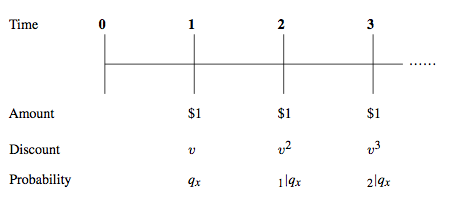
\includegraphics[width=0.8\linewidth]{fig1.png}
    \caption{Discrete whole life insurance}
\end{figure}






Then the expected present value of the benefit is:
\begin{align}
A_x = \text{E}[v^{K_x+1}] = \sum_{k=0}^{\infty} v^{k+1}*_{k\mid} q_x  \nonumber 
\end{align}

$_{k\mid} q_x$ stands for the probability that a life aged $x$ survived $k$ years, now $x+k$ years old, will die in the next subsequent year.

\textbf{Whole life annuity-due}: Denoted $\ddot{a}_x$. Consider a whole life annuity with \pounds1 payable yearly in advanece to an annuitant aged $x$, and the annuitant dies between year $K_x$ and $K_x+1$, see the chart below



\begin{figure}[H]
    \centering
    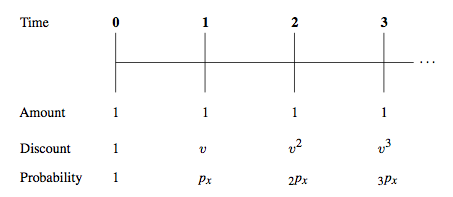
\includegraphics[width=0.8\linewidth]{fig2.png}
    \caption{Whole life annuity-due}
\end{figure}


\section{Pricing}


Then the expected present value of the payments is :
\begin{align}
        \ddot{a}_x&= 1 + vp_x +v^2_2p_x +v^3_3p_x+ \dots\nonumber 
\end{align}
\text{that is} 
\begin{align}
        \ddot{a}_x&= \sum_{k=0}^{\infty} v^k*_kp_x = \frac{1-A_x}{d} \nonumber 
\end{align}
where $d=\frac{i}{(1+i)}$





Now the last unknown parameter has obtained, we can proceed to the next step, calculating expected present value of renewal expenses and future payments.



Recall from last section, the single premium $P$ equals to the liabilities in the future, which including three parts: initial expense, the EPV of renewal expenses and EPV of future payments.


Let us start from calculate the EPV of renewal expenses
\subsubsection{EPV of renewal expenses}

Recall equation (1.2)

\begin{align}
        \text{EPV of renewal expense}&= R  * \sum_{t=1}^{\infty}(1 + c )^{t-1} * _tp_{[x]}* v^t \nonumber \\
        &= \frac{R}{(1+c)} * \sum_{t=1}^{\infty} (1 + c )^t * _tp_{[x]} * v^t \nonumber \\
        &= \frac{R}{(1+c)} * \sum_{t=1}^{\infty} [(1 + c )*v]^t * _tp_{[x]} \nonumber \\
\text{given $v$ = $\frac{1}{(1+i)} $}\nonumber \\
        &= \frac{R}{(1+c)} * \sum_{t=1}^{\infty} \left(\frac{1+c}{1+i}\right)^t * _tp_{[x]} \nonumber \\
\text{let $v_j = \frac{1+c}{1+i}$, now we have}\nonumber \\
        &= \frac{R}{(1+c)} * \sum_{t=1}^{\infty} v_j^t * _tp_{[x]} \\
        &= \frac{R}{(1+c)} * (\ddot{a}_{[x]j}-1)
\end{align}

\textbf{Notes:}
\begin{itemize}
\item $\ddot{a}_{[x]j}$ is the annuity with changed discount rate from $v$ to $j$,  $\ddot{a}_{[x]j} = \sum_{t=0}^{\infty} v_j^t * _tp_{[x]}$
\item We have $\ddot{a}_{[x]j} - 1$ here is because the renewal expense will not be applied in the first year.
\end{itemize}

\subsubsection{EPV of future payments}
\begin{align}
        \text{EPV of future payments} &= S * \sum_{t=10}^{\infty} (1 + c )^{t-10} * _tp_{[x]} * v^t \nonumber \\
         &= \frac{S}{(1+c)^{10}}* \sum_{t=10}^{\infty} (1 + c )^{t} * _tp_{[x]} * v^t \nonumber \\
         &= \frac{S}{(1+c)^{10}} * \sum_{t=10}^{\infty} v_j^t * _tp_{[x]}
\end{align}

\textbf{Note:}
\begin{itemize}
\item For both of the expected present value of expenses and future payments, the summation will be up till $120-x$ instead of $\infty$ when we model them, this is based on our assumption that all lives will cease before age 120. 
\end{itemize}



To calculate both equation (1.4) and (1.6), the easiest way is programming. Here I use C++ \footnote{Codes will be included in appendix} generated 1,000 pseudo random numbers between 55 and 60 reprensent the age of the anntuitant, F or M represent the gender and Y or N represent smoking habit. For each of them in the group the single premium will be calculated using different mortality rate tables depend on the three factors. We set a non-smoking female annuitant age 55 as a example.
\begin{align}
        \text{EPV of renewal expense}&= \frac{R}{(1+c)} * \sum_{t=1}^{\infty} v_j^t * _tp_{[x]} \nonumber \\
         &= \frac{30}{(1+0.028)} * \sum_{t=1}^{\infty} 0.98^t * _tp_{[55]} \nonumber\\
         &= 539.88\nonumber\\
        \text{EPV of future payments} &= \frac{50,000}{(1+0.028)^{10}} * \sum_{t=10}^{\infty} 0.98^t * _tp_{[55]} \nonumber\\ 
         &=549,941.32 \nonumber
\end{align}

Therefore, the single premium for a $55$ non-smoking female annuitant will be 
\begin{align}
500 + 539.88 +549,491.32= \pounds550,981.2 \nonumber
\end{align}

For the 1,000 annuitant, the accumulated single premiums insurer can obtain is 606,029,320.

\subsection{Profitablity}

In the last section, we had obtained the premium for the target annuitants, now the insurer would want to know the probability that the company can make profit on the contract and the probability the loss will exceed a certain amount.

Continue on the previous example, we use the loss random variable again to denote the loss at year t:

\[
 L_0(t) =
  \begin{cases}
   -P + 500 + \frac{30}{(1+0.028)} * \sum_{t=1}^{\infty} 0.98^t * _tp_{[55]} & \text{for } t= 0,1, \dots, 9 \\
   -P +500 +539.88 +  50,000*v^{10}*\ddot{a}_{x-9,j}  & \text{for }  t = 10, 11\dots
  \end{cases}
\]

where $j= \frac{1+0.05}{(1+0.028)}-1=0.0214$

The expected present value of the profit will be positive if $L_0(t) < 0$, therefore
 \begin{align*}
   -550,981.2 +500+ 539.88 + 50,000*v^{10}*\ddot{a}_{x-9,j}  &< 0 \\
   50,000*v^{10}*\ddot{a}_{x-9,j} &< 549,941.32 \\
   \ddot{a}_{x-9,j} &< 17.92 \\
\text{Rewrite } \ddot{a}_{x-9,j} = \frac{1-v^{t-9}_j}{d_j} \text{ where } d_j =\frac{j}{1+j}\\
\text{rearrange we will obtain}\\
v^{t-9}_j &> 1-d_j\times 17.92\\
v^{t-9}_j &> 0.625\\
\text{we have } v_j = exp\{-\delta_j\} \text{and } \delta_j =log(1+j),\text{therefore}\\
t-9&< \frac{-log(0.625)}{\delta_j}\\
\text{and } t &< 31.2
\end{align*}

In another words, if the select 55-year-old female non-smoking annuitant survive no more than 31 years, this company will make profit. 

For risk management, the company would like to know the probability that the loss exceed \pounds50,000 and \pounds100,000. We can use the same loss random variable to achieve this:

 \begin{align*}
   -550,981.2 +500+ 539.88 + 50,000*v^{10}*\ddot{a}_{x-9,j}  &< 50,000 \\
\text{and}\\
-550,981.2 +500+ 539.88 + 50,000*v^{10}*\ddot{a}_{x-9,j}  &< 100,000 
\end{align*}

Following the same steps, we can obtain that for loss exceed \pounds50,000, the annuitant will have to survive to age 88 years old with probability $_{33}p_{[55]} = 0.42$, and for loss exceed \pounds100,000 the annuitant will have to survive at least 36 years to 91 with probability $_{36}p_{[55]} = 0.37$. 


\section{Sensitivity test}

\subsection{Change in mortality rate}



\subsection{Change in inflation rate}























\chapter{Unit-linked insurance}     \label{unit-linked}



In this chapter we are going to introduce the unit-linked insurance contract. Starting from some assumptions to construct a deterministic pricing model, we demonstrate that the deterministic pricing test is not accurate enough for this contract.
% Do not understand.
This is because the uncertainty, or in other words risk, in the investment is not diversifiable.  

To solve this problem, a stochastic pricing test will be considered, with the future return on the investment modelled as a random variable, and then a sensitivity test will be used again to find the best assumption for this contract and determine the reserve. 


\section{Background}

In some countries the unit-linked contract is also called an equity-linked contract. This is because the single or regular premium paid by the policy holder will be invested on units of equity or bonds on their behalf. Once the insurer receives the premium, it will be paid into the policy holder's fund after deduction of expenses and management costs in that year, and the deduction goes to insurer's account. In UK, there is an un-allocated percentage, which is another agreed regular deduction from the policy holder's fund to insurer's account.

If the policy holder survives to the maturity date, they will receive the greater value between accumulated premiums paid and the fund in policy holder's account. This is called guaranteed minimum maturity benefit (GMMB) \cite{bib:GMMB}. But the if the death happens first, there is a guaranteed minimum death benefit, which allows policy holder's estate to receive the policy holder's fund with an extra amount, e.g. 10\% extra of the policy holder's fund. 


\subsection{Some assumptions}  \label{unit-link-basic-assumptions}

Before we establish the model, we need some assumptions, the following are some ideas from  \cite{bib:unitlinkeg} book {\em Actuarial Mathematics for Life Contingent Risks,} and some online sources \cite{bib:unitlinkedonline}. 


A company is going to issue a new 10 year unit-linked contract to people aged 55 to 60. In the contract, it stated that the annual premium is \textsterling 5200, with an un-allocated rate of 5\% in the first year and 1\% in the subsequent years. This will be deducted immediately after the insurer receives the premium. Expenses occurs the same time as the premium is paid in, which is 13\% (including commission) and 0.7\% respectively. At the end of each year, there is a further management charge of 0.8\%  discounted from the policy holder's fund. The deductions from the policy holder's account will be transferred to the insurer's account.

When the contract matures, the policy holder can receive the greater value between policy holder's fund and accumulation of premiums paid. But if the death happens before the maturity date, the policy holder's estate will receive 110\% of the policy holder's fund where the extra 10\% is from the insurer's account.

The insurance company is also prepared to have 10\% of policy holders surrender the contract in the first year and 5\% in the second year, but no more in the subsequent years. The policy holders who surrender the contract will receive their premium(s) after the deducted management cost at the end of the year.

In the Chapter \ref{annuity}, we introduced different methods to calculate the mortality rate, but here we are going to use a constant force of mortality, $\mu_x=2.2218$, for people aged 55 to 60, which means the mortality rate of policy holders is $q_x=0.006$ in each year\footnote{$q_x$= exp $\left\{-\int_0^1 \mu_{x+s}ds\right\}$}. The reason we set the mortality rate to a constant will be explained later in this chapter.  





\section{Deterministic pricing and reserving}

% Needs rephrasing
In the previous section we introduced the unit-linked contract, and gave some assumptions to construct the model. But there is something has not been counted in: the uncertainty in the investment return in policy holder's account and insurer's account. 

For deterministic pricing, we used conservative interest rates for both accounts, 8\% for the policy holder's account and 5\% for the insurer's account, and assume no reserve holds in this case. Since the mortality rate is a constant, as well as the conservative interest rates, the cash flow for different policy holders will be exactly the same. Here is one example.

\subsection{Cash flow}

From all the assumptions, cash flow tables for both the policy holder and insurer's account for the  10 year term can be easily constructed. Let us explore the policy holder's account first. 



\begin{figure}[H]
    \centering
\begin{tabular}{p{1cm} p{1.5cm} p{1.5cm} p{2cm} p{1.5cm} p{2cm} p{1.5cm} p{1.5cm} }
\toprule
\multicolumn{8}{c}{Cash flow for policy holder's account} \\
\cmidrule(r){3-7}

Year t & Annual premium & Allocated premium & Fund brought forward & Interest & Fund at time $t^-$ & Manage-ment cost & Fund bring forward \\
\midrule
1	&5,200	&4,940	&0&	395.2	&5,335.2	&42.68	&5,292.52\\
2	&5,200	&5,148	&5,292.52	 &   835.24	&11,275.76 &	90.21	&11,185.55\\
3	&5,200	&5,148	&11,185.55&  1,306.68	&17,640.24	&141.12  &17,499.12\\
4&	5,200	&5,148	&17,499.12&  1,811.77&	24,458.89	&    195.67       &24,263.21\\
5&	5,20,0	&5,148&	24,263.21	&    2,352.89&	31,764.11	&   254.11	&31,509.99\\
6&	5,200	&5,148&	31,509.99	&   2,932.64&	39,590.64	&   316.73	&39,273.91\\
7&	5,200	&5,148&	39,273.91	&   3,553.75&	47,975.67	&   383.81	&47,591.86\\
8&	5,200	&5,148&	47,591.86	&   4,219.19&	56,959.05	&  455.67	    &56,503.38\\
9&	5,200	&5,148&	56,503.38	&   4,932.11&	66,583.49	&  532.67 	&66,050.82\\
10&	5,200	&5,148	&66,050.82	&5,695.91	&76,894.73	&615.16	&76,279.57\\
\bottomrule
\end{tabular}
\label{determ-PHcashflow}
\caption{Deterministic cash flow in one policy holder's account}
\end{figure}




\textbf{Notes:} Here is how the cash flow table been calculated.

\textbf{Allocated premium:} For the first year, the allocated premium in the policy holder's fund will be (1-5\%) of the total premium paid, and the other 5\% is the agreed un-allocated premium which will be paid into insurer's account. For the subsequent years, the un-allocated rate decrease to 1\%, hence there will be 99\% premium paid into policy holder's fund.


First year allocated premium:                5,200 $\times$ 0.95 = 4,940

Subsequent years allocated premium:   5,200 $\times$ 0.99 = 5,148


\textbf{Interest:} This is the 8\% interest that the policy holder obtains from the accumulation of the premium paid in at the beginning of the year and fund brought forward from last year.

e.g.  year t=5, interest = (5,148 + 24263.21) $\times$ 0.08 = 2,352.89

\textbf{Fund at time $t^-$:} This is the fund in policy holder's account after interest paid in.

\textbf{Management cost:} In our assumption, the management cost is 0.08\% of the policy holder's fund, which is the fund at time $t^-$ in our case. 

\textbf{Fund bring forward:} This is the fund left in policy holder's account after deduction of management cost. 


Table \ref{determ-insurer} is showing the insurer's account cash flow for \textbf{one} policy holder\footnote{If there are $N$ policy holders, then the numbers in the table times $N$ will be the cash flow for the insurer in 10 years}. 


\begin{figure}[H]
\hfill
    \centering
\begin{tabular}{p{0.8cm} p{1.5cm} p{1.5cm} p{1.2cm} p{1cm} p{2cm}p{1.5cm} p{1.5cm} p{1.5cm} }
\toprule
\multicolumn{9}{c}{Cash flow for insurer's account} \\
\cmidrule(r){3-7}

Year t & Annual premium & Un-allocated premium & Expenses & Interest &Management cost& Expected death benefit & Profit& $\Pi_t$  \\
\midrule

0&0&0&676&0&0&0&-676&-676\\
1&5,200&260&36.4&11.18&42.686&3.18&274.29&274.29\\
2&5,200&52&36.4&0.78&90.21&6.71&99.87&89.35\\
3&5,200&52&36.4&0.78&141.12&10.50&147.00&124.14\\
4&5,200&52&36.4&0.78&195.67&14.56&197.49&165.78\\
5&5,200&52&36.4&0.78&254.11&18.91&251.59&209.92\\
6&5,200&52&36.4&0.78&316.73&23.56&309.54&256.73\\
7&5,200&52&36.4&0.78&383.81&28.56&371.63&306.38\\
8&5,200&52&36.4&0.78&455.67&33.90&438.15&359.05\\
9&5,200&52&36.4&0.78&532.67&39.63&509.42&414.95\\
10&5,200&52&36.4&0.78&615.16&45.77&585.77&474.28\\

\bottomrule
\end{tabular}
\caption{Deterministic cash flow in insurer's account}
\label{determ-insurer}
\end{figure}

\textbf{Notes:}

In insurer's account, un-allocated premium, expense, interest and management cost are calculated in the same way as in policy holder's account. You may notice there is an extra row in the table, year 0 in insurer's cash flow, this is the acquisition expense which will always occur before the insurer receives the premium, e.g. commission, renting, employees.

For expected death benefit, profit and profit signature are calculated as below:

\textbf{Expected death benefit:} If the death occurs before the contract matures, the policy holder's estate will receive 110\% of the policy holder's fund where the extra 10\% is from insurer account. The death benefit we calculate here is the 10\% from the insurer's account. 

\textbf{At time 0}, the policy holder has just entered the contract and so the probability for the contract to be in force is 1.

\textbf{In year 1}, policy holders pay the first premium right after they sign the contract, so the probability for the contract to be in force is still 1. 

\textbf{During the first year}, by our assumption, 10\% policy holders surrender the contract, and the mortality rate for the other 90\% is 0.006. Therefore, at the beginning of the second calendar year, insurer will be expecting $p_2= (1-0.006) \times(1-0.1)$ =0.8946 of policy holders to renew their contracts. 

\textbf{At the beginning of third year}, the insurer will be expecting $p_3= (1-0.006-0.5) \times p_2$= 0.8445024 of policy holders renew the contract, since by assumption 5\% of policy holder will surrender during the second year.

From the third year, the probability for the contract to be in force will be $p_t = (1-0.006) \times p_{t-1}$. (Showing in table \ref{determ-prob-in-force}.)


\begin{figure}[H]
    \centering
\begin{tabular}{|l|l|}
  \hline
  \multicolumn{2}{|c|}{probability in force} \\
  \hline
t=	& $_t p_x$\\
\hline
0	&1\\
1	&1\\
2	&0.8946\\
3	&0.8445024\\
4	&0.839435386\\
5	&0.834398773\\
6	&0.829392381\\
7	&0.824416026\\
8	&0.81946953\\
9	&0.814552713\\
10	&0.809665397\\
  \hline
\end{tabular}
\caption{Probability for the contract in force}
\label{determ-prob-in-force}
\end{figure}


\textbf{Profit:} For each year, profit is calculated by the formula

Profit = Un-allocated premium - Expenses + Interest + Management cost - Death benefit

\textbf{Profit signature:} This is profit the insurer can make with probability that the contracts are still in force, which is defined as $\Pi_t = p_x \times Profit_t$


\subsection{Profitability}


From the figure \ref{determ-PHcashflow}, there is obviously an ascending trend on the policy holder's fund, and on the contract maturity date, it reaches \pounds 76,279, which is approximately 1.47 times of the accumulation of all premiums. This means, if the policy holder survives to the maturity date, he/she will withdraw the policy holder's fund since it will always be the greater one compared to the accumulation of all the premiums. \footnote{GMMB policy: on the maturity date policy holders can withdraw the greater value between policy holder's fund and the accumulation of all the premiums paid.} This means the insurer will have a probability of 0.81 \footnote{The probability that this contract is in force until the maturity date is showing in figure\ref{determ-prob-in-force}.} to make profit of \pounds 585.77 on each policy holder. And if we discount the profit signature with the risk discount rate of interest of 15\%, the net present value of the profit will be 
\[
 NPV=\sum_{i=1}^{10} \Pi_t \times (1+0.15)^{-t} = \pounds 489.59
\]
 
and the profit margin will be


\[
\text{Profit\ Margin} =  \frac{NPV}{P \ddot{a}_x} = 1.24\%
\]

<<<<<<< HEAD
where $\ddot{a}_x$=$\sum_{i=1}^{10} v^t {_tp_x}$=7.619285226, where $_tp_x$
read from table ?!?!?!? and $v=\frac{1}{1+0.05}$  = $\frac{489.59}{5200 \times
7.619285226}$
=======
where $\ddot{a}_x$=$\sum_{i=1}^{10} v^t {_tp_x}$=7.619285226, where $_tp_x$ read from table ?!?!?!? and $v=\frac{1}{1+0.05}$  = $\frac{489.59}{5200} \times 7.619285226$
>>>>>>> thx Antony!

Since in the very beginning, we used conservative assumptions, e.g. expenses, mortality rate, interest rate for the insurer's fund. So if in reality the expense and mortality rate are lower than modelled and the interest rate is higher, then the insurer will obtain more profit. A sensitivity test can be used here to show how the profit changes with according to different factors. 

\subsection{Sensitivity test}

Now we change our previous assumptions one by one and see what will happen.

\textbf{Scenario 1: Lower expenses} 

The initial expense deduction changed from 13\% to 10\%, and the renewal changed from 0.7\% to 0.5\%.




\begin{figure}[H]
\hfill
    \centering
\begin{tabular}{p{0.8cm} p{1.5cm} p{1.5cm} p{1.2cm} p{1cm} p{2cm}p{1.5cm} p{1.5cm} p{1.5cm} }
\toprule
\multicolumn{9}{c}{Cash flow for insurer's account} \\
\cmidrule(r){3-7}

Year t & Annual premium & Un-allocated premium & Expenses & Interest &Management cost& Expected death benefit & Profit& $\Pi_t$  \\
\midrule

0&0&0&520&0&0&0&-520&-520\\
1&5200&260&26&11.7&42.68&3.18&285.21&285.21\\
2&5200&52&26&1.3&90.21&6.71&110.80&99.12\\
3&5200&52&26&1.3&141.12&10.50&157.92&133.37\\
4&5200&52&26&1.3&195.67&14.56&208.41&174.95\\
5&5200&52&26&1.3&254.11&18.91&262.51&219.035\\
6&5200&52&26&1.3&316.73&23.56&320.46&265.79\\
7&5200&52&26&1.3&383.81&28.56&382.55&315.38\\
8&5200&52&26&1.3&455.67&33.90&449.07&367.99\\
9&5200&52&26&1.3&532.67&39.63&520.34&423.84\\
10&5200&52&26&1.3&615.16&45.77&\textbf{596.69}&\textbf{483.12}\\

\bottomrule
\end{tabular}
\caption{Sensitivity test for a lower expense rate}
\label{determ-sensi-expense}
\end{figure}

The table shows the profit increased about \pounds 10 on the maturity date, and the new NPV of profit becomes 

\[
 NPV=\sum_{i=1}^{10} \Pi_t \times (1+0.15)^{-t} = \pounds693.24 
\]
 
and the profit margin is:

\[
\text{Profit Margin} =  \frac{NPV}{P \ddot{a}_x}= \frac{693.24 }{5200 \times 7.619285226} = 1.7\%
\]

$\ddot{a}_x$=$\sum_{i=1}^{10} v^t {_tp_x}$=7.619285226, where $_tp_x$ read from table ?!?!?!? and $v=\frac{1}{1+0.05}$ 

This shows if we can lower the cost in the company, then more profit can be made, However, in reality, this is really hard to achieve, since some certain costs are unavoidable, e.g. renting, salary.




\textbf{Scenario 2: Lower mortality rate} 

Constant mortality rate change from 0.006 to 0.005.



\begin{figure}[H]
\hfill
    \centering
\begin{tabular}{p{0.8cm} p{1.5cm} p{1.5cm} p{1.2cm} p{1cm} p{2cm}p{1.5cm} p{1.5cm} p{1.5cm} }
\toprule
\multicolumn{9}{c}{Cash flow for insurer's account} \\
\cmidrule(r){3-7}

Year t & Annual premium & Un-allocated premium & Expenses & Interest &Management cost& Expected death benefit & Profit& $\Pi_t$  \\
\midrule

1&5,200&260&36.4&11.18&42.68&2.65&274.82&274.81\\
2&5,200&52&36.4&0.78&90.21&5.59&100.99&90.44\\
3&5,200&52&36.4&0.78&141.12&8.75&148.75&125.88\\
4&5,200&52&36.4&0.78&195.67&12.13&199.92&168.34\\
5&5,200&52&36.4&0.78&254.11&15.75&254.74&213.42\\
6&5,200&52&36.4&0.78&316.73&19.64&313.47&261.31\\
7&5,200&52&36.4&0.78&383.81&23.80&376.39&312.20\\
8&5,200&52&36.4&0.78&455.67&28.25&443.80&366.27\\
9&5,200&52&36.4&0.78&532.67&33.03&516.02&423.74\\
10&5,200&52&36.4&0.78&615.16&38.14&\textbf{593.40}&\textbf{484.85}\\

\bottomrule
\end{tabular}
\caption{Sensitivity test for mortality rate change}
\label{determ-sensi-morta}
\end{figure}

Here are the new net present values of profit and profit margin obtained from the new cash flow:
\[
 NPV=\sum_{i=1}^{10} \Pi_t \times (1+0.15)^{-t} = \pounds 491.43
\]
 


\[
\text{Profit Margin} =  \frac{NPV}{P \ddot{a}_x}= \frac{491.43}{5200 \times 7.619285226} = 1.24\%
\]

$\ddot{a}_x$=$\sum_{i=1}^{10} v^t {_tp_x}$=7.619285226, where $_tp_x$ read from table ?!?!?!? and $v=\frac{1}{1+0.05}$


The lower mortality rate will only affect the insurer's account. The table shows that the profit will increase from \pounds585.77 to \pounds 593.40, the raise in net present value of the profit is less than \pounds2, and the profit margin will not change. This means the change in mortality rate is not sensitive, and should not be counted as an important factor in our model, so a constant assumption for the mortality rate is acceptable.



\textbf{Scenario 3: Higher interest rate} 

Interest rate change from 8\% to 9\%.


\begin{figure}[H]
    \centering
\begin{tabular}{p{1cm} p{1.5cm} p{2cm} p{2cm} p{1cm} p{1.5cm} p{1.5cm} p{1.5cm} }
\toprule
\multicolumn{8}{c}{Cash flow for policy holder and insurer's account} \\
\cmidrule(r){3-7}

Year t & Interest &Fund at time $t^-$ & Management cost  & Fund bring forward & & Profit& $\Pi_t$ \\
\midrule
0&&&&&&-676&-676\\
1&444.6&5,384.6&43.08&5,341.5232&&274.65&274.65\\
2&944.06&11,433.58&91.47&11,342.11&&101.04&90.39\\
3&1,484.11&17,974.22&143.79&17,830.43&&149.48&126.23\\
4&2,068.06&25,046.49&200.37&24,846.11&&201.84&169.44\\
5&2,699.47&32,693.58&261.55&32,432.04&&258.47&215.67\\
6&3,382.20&40,962.24&327.7&40,634.54&&319.7&265.15\\
7&4,120.43&49,902.97&399.22&49,503.75&&385.9&318.14\\
8&4,918.66&59,570.4&476.56&59,093.84&&457.49&374.9\\
9&5,781.77&70,023.6&560.19&69,463.42&&534.89&435.67\\
10&6,715.03&81,326.44&650.61&\textbf{80,675.83}&&\text{618.59}&500.85\\
\bottomrule
\end{tabular}
\caption{Sensitivity test for interest rate change}
\label{determ-sensi-interest}
\end{figure}


In the table, it shows that once the interest increases by 1\%, the fund in the policy holder's account will increase by about 4.6\% every year, the profit for insurer will increase 5.3\% on the date of maturity. In addition, the new net present value of profit and will be:

\[
 NPV=\sum_{i=1}^{10} \Pi_t \times (1+0.15)^{-t} = \pounds522.72
\]
 
The profit margin becomes:


\[
\text{Profit Margin} =  \frac{NPV}{P \ddot{a}_x} = \frac{522.72}{5200 \times 7.619285226} = 1.3\%
\]

There is a big raise in both NPV of profit and profit margin. NPV of profit increases from \pounds489.59 to \pounds522.72, and the profit margin shoots up from 1.24\% to 1.3\%. This is a very sensitive case, where a small change in interest will have a huge impact in profit. Therefore a good interest model will be very essential in this case.
 





\subsection{Short summary for deterministic test}
So far everything looks fine, but is this a good model for a unit-linked contract? The answer will be no, since from our sensitivity test, we can see that the interest rate change will lead to a huge fluctuation in profit, so the assumption of a constant interest rate is not good enough in this case. This is because the constant interest rate does not contain  enough information when modelling, since the uncertainty of investment on equity and bond is not diversifiable. By law, we do not have an arbitrage market, no one can make profit without risk, and the interest on return will be affected by a few different factors, \cite{bib:riskfactor} e.g. inflation, quality of information, governmental policy, change in bond market or equity market. Once the factors  are affecting the market at the same time, the risk will be non-diversifiable. So now we should consider modelling the interest rate non-linearly, e.g. as a random variable. 




\section{Stochastic pricing}

From the sensitivity test in the last section, we conclude that the change in interest rate is non-diversifiable and extremely sensitive, so a constant assumption is not suitable. 
For a more realistic model we introduce the stochastic price test. Here, we model the interest rate as a random variable, avoiding the constant assumption of the previous section.


\subsection{Central Limit Theorem and Monte Carlo simulation}

In our basic assumptions \footnote{assumption in \ref{unit-link-basic-assumptions}}, we assume that the policy holders will be able to choose different units of equities or bonds or portfolios \footnote{Portfolio: mixed equities and bonds} to invest their premium. This means that the more equities and bonds available, the less similarity in the interest return each year for different policy holders. 

By \cite{bib:CLT}the Central Limit Theorem, which obtained by Mood, Graybill, and Boes in 1974, if we have a number of independent identically distributed random variables \footnote{The random variables can follow any distribution}, we can observe a new series of random variables following the normal distribution by summing or multiplying the old ones. The theorem can be used in finance, compound return or equity return which follows a log-normal distribution\footnote{log-normal distribution is also called Galton's distribution, after Francis Galton}, which means the logarithm of interest return $I_t$ follows a normal distribution with mean $\mu$ and variance $\sigma^2$. This theorem can be applied in the new model, then we will have
\[
logI_t  \sim N(\mu,\sigma^2)
\]
\[
\text{where}   \mu= 0.74928, \sigma= 0.15 
\]

Now we can use Monte Carlo simulation\cite{bib:MCS}, generate some (pseudo) random numbers \footnote{I used C++ boost random number generator.} $\xi'_t$ from the Standard Normal distribution with mean 0 and variance 1, and transform them to the specified Normal distribution $N(0.74928,0.15^2)$ via   
\[
\xi_t = 0.74928 + 0.15\times \xi'_t
\]
Then, our annual accumulation\footnote{It is the interest rate $r_t$ + 1} factor will be simulated by 
\[
I_t=exp\{\xi_t\} 
\]



\subsection{Modelling}

Now we assume there are 1,000 policy holders \footnote{The larger number the better statistic result we will get, here we just set 1,000 as an example.} purchased unit-linked contract with different portfolios. Using the generated random variable from the Standard Normal distribution, we can construct our new cash flow tables. I used C++ to help me with constructing the tables \footnote{codes will be included in the appendix}. Since there are 1,000 policy holdders and interest rate will be different from year to year for all of them. Therefore, 10,000  $\xi'_t$ need to be generated from the Standard Normal distribution.


Here is an example we get from the program. \footnote{To curious readers, this is the 1st cash flow table we get from the program.}


\begin{figure}[H]
    \centering
\begin{tabular}{p{0.5cm} p{1.5cm} p{1.3cm} p{1cm} p{1.5cm} p{1.2cm} p{1.3cm} p{1.3cm}p{1.3cm}p{1.3cm}p{1.3cm} }
\toprule
\multicolumn{10}{c}{Cash flow for policy holder and insurer's fund} \\
\cmidrule(r){3-8}

Year t & $\xi_t$ &$R_t$ & Prem-ium & Alloc-ated Premium & Fund at $t^-$ &Manage-ment & Fund at t& Profit& $\Pi_t$ \\
\midrule
0&0&0&0&0&0&0&0&-676&-676\\
1&0.213436&1.11287&5,200&4,940&5,497.58&43.9807&5,453.6&313.709&313.71\\
2&-0.49558&1.00059&5,200&5,148&10,607.9&84.863&10,523&94.9292&84.92\\
3&1.57538&1.36511&5,200&5,148&21,392.6&171.141&21,221.5&174.788&147.61\\
4&-1.0592&\textbf{0.919475}&5,200&5,148&\textbf{24,246.1}&193.969&\textbf{24,052.1}&195.917&164.46\\
5&1.83927&1.42023&5,200&5,148&41,470.8&331.767&41,139.1&323.463&269.90\\
6&1.88577&1.43017&5,200&5,148&66,198.4&529.587&65,668.8&506.566&420.14\\
7&0.604675&1.18014&5,200&5,148&83,573.4&668.588&82,904.9&635.225&523.69\\
8&-0.365983&1.02023&5,200&5,148&89,834.4&718.675&89,115.7&681.586&558.54\\
9&-0.578264&0.988258&5,200&5,148&93,156.9&745.255&92,411.6&706.188&575.22\\
10&-0.634376&0.979975&5,200&5,148&95,606&764.848&94,841.1&724.323&586.46\\

\bottomrule
\end{tabular}
\caption{Stochastic cash flow 1}
\label{stoch-cashflow}
\end{figure}

\textbf{Notes:}

\textbf{$\xi_t$:} This column is the generated random variables from Standard Normal distribution.

\textbf{$R_t$:} This is simulated annual accumulation factor, \textbf{the annual interest rate} is $r_t = R_t -1$.

\textbf{Other columns in the table:} The table was calculated using the same method in deterministic cash flow, the only difference is the interest rate had changed.


From the table \ref{stoch-cashflow} we can see that, the annual accumulation factor is sometimes less than one, which indecates that annual interest $r_t = R_t - 1$ is negative, then there is a loss in the policy holder's fund in that year. But for the insurer in this case, the net present value of profit and profit margin\footnote{Profit margin is calculated using risk discount factor 15\%.} are ideal: 

\[
NPV=\pounds 1,011.86\ \ \ \   \   \& \    \ \ \ \       Profit \  margin = 2.6\%
\]

Now showing another example from the 1,000 which is not that ideal for the insurer.

\begin{figure}[H]
    \centering
\begin{tabular}{p{0.5cm} p{1.5cm} p{1.3cm} p{1cm} p{1.5cm} p{1.2cm} p{1.3cm} p{1.3cm}p{1.6cm}p{1.5cm}p{1.3cm} }
\toprule
\multicolumn{10}{c}{Cash flow for policy holder and insurer's fund} \\
\cmidrule(r){3-8}

Year t & $\xi_t$ &$R_t$ & Prem-ium & Alloc-ated Premium & Fund at $t^-$ &Manage-ment & Fund at t& Profit& $\Pi_t$ \\
\midrule
0&0&0&0&0&0&0&0&-676&-676\\
1&-1.33578&0.88211&5,200&4,940&4357.62&34.86&4,322.76&305.27&305.27\\
2&-0.412251&1.01318&5,200&5,148&9,595.55&76.76&9518.79&87.43&78.22\\
3&-1.09414&0.91467&5,200&5,148&13,415.3&107.32&13,307.9&115.72&97.72\\
4&0.847198&1.22386&5,200&5,148&22,587.4&180.7&22,406.7&183.64&154.15\\
5&-0.581987&0.987706&5,200&5,148&27,216&217.73&26,998.3&217.91&181.82\\
6&0.43257&1.15006&5,200&5148&36,970.1&295.76&36,674.3&290.14&240.64\\
7&0.0178033&1.08069&5,200&5148&45,196.9&361.58&44,835.4&351.05&289.412\\
8&-2.10093&0.786462&5,200&5148&39,310&314.48&38,995.5&307.46&251.96\\
9&-1.4693&0.864618&5,200&5148&38,167.3&305.34&37,862&299.00&243.55\\
\textbf{10$^*$}&-0.207703&1.04474&5,200&5148&44,934.4&359.48&\textbf{44,575}&\textbf{349.11}&-4,609.47\\
\textbf{10}&-0.207703&1.04474&5,200&5148&44,934.4&359.48&\textbf{44,575}&\textbf{-7,031.38}&-5,693.06\\

\bottomrule
\end{tabular}
\caption{Stochastic cash flow2}
\label{stoch-cashflow}
\end{figure}


\textbf{Note:}


\textbf{Row 10$^*$ \& 10:} It is showing that the fund in policy holder's account at the mature date, \pounds 4,4575, is less than the accumalation of 10 premiums, \pounds 52,000, therefore the difference will be deducted to pay off the insurer's liability with probability 0.994\footnote{The probability that the contract is still in force from year 9, table \ref{determ-prob-in-force}.}. 
\[
(52,000- 44,575)\times 0.994= \pounds 7,380.45 
\]
The profit showing in row $10^*$ is the profit in year 10 before the deduction, the actual profit the insurer obtaind at the mature date is \pounds349.11 - \pounds7,380.45 = -\pounds 7031.3 showing in row 10. And the NPV of the profit in this case is -\pounds995.422, and the profit margin is $-2.5\%$.



Now there are two examples for both situation, making profit and lossing, it will be really important for the company to know the statistic numbers, e.g. how many contracts have negative NPV of profit, how much profit can the company make, what is the probability for the company to lose etc..

\subsection{Statistic analysis}

In the C$^{++}$ program, the NPV can be sorted in order, and counted how many negative values are there, the table below showing the statistic results. 

\texttt{NPV median = 677.104}

{\renewcommand\baselinestretch{1}\selectfont


\texttt{NPV fifth percentile = \textbf{-927.485}}

\texttt{NPV ninety fifth percentile = 1035.04}

\texttt{NPV mean = 534.232}

\texttt{NPV sd = 687.702}

\texttt{NPV count negative values = \textbf{85}}

\texttt{95\% CI for NPV = (491.607,576.856)}
\par}

\textbf{Notes:} 

\textbf{NPV median:} This is the sample median of all NPV of profit.

\textbf{NPV 5$^{th}$ percentile:} The 50$^{th}$ in the ascending order 1,000 NPV of profit.

\textbf{NPV 95$^{th}$ percentile:} The 950$^{th}$ in the ascending order 1,000 NPV of profit.

\textbf{NPV mean:} This is the sample mean, which calculated by $\frac{\sum_{i=1}^{1000} NPV_i}{1000}$

\textbf{NPV sd:} This is the sample standard deviation. 

\textbf{NPV count negative values:} This is the number of negative NPV of profit out of 1,000.

\textbf{95\% CI for NPV:} The 95\% of all NPV of profit will drop in this interval.


There are 85 negative NPV of profit out of 1,000, which means the probability for this company to lose on this contract is 8.5\%, which is considerablely high. And the 5$^{th}$ percentile, ${-\pounds927.485}$, is a very large lose as well. In conclusion, this contract has a high probability of losing a large amount of money, which should not be issued in reality. This is caused by the gauranteed benefit increased the risk for insurer. In the next section we are going to disscuss how to lower the risk and make a profit.


\subsection{Stochastic pricing}

Recall in Chapter \ref{annuity}, the equivalence principle were used to find the premium, but it can not be used in this unit-linked contract since there is a non-diversifiable risk. But instead, we can use stochastic simulation with quantile premium principle\cite{bib:quantile-premium}. 

For quantile premium principle, the idea is to obtain a profit with a certain probability. If the $5^{th}$ percentile is positive and probability of loss is no greater than 5\% then it is a good model and can be taken to practice. Based on the previous model, changing in some assumptions may let us achieve this target. 

\textbf{Scenario 1: Increase the premium}

Increase the premium from \pounds5,200 to \pounds5,400

\texttt{NPV median = 703.147}

{\renewcommand\baselinestretch{1}\selectfont

\texttt{NPV fifth percentile = \textbf{-963.16}}

\texttt{NPV ninety fifth percentile = 1074.85}

\texttt{NPV mean = 554.779}

\texttt{NPV sd = 714.152}

\texttt{NPV count negative values = \textbf{85}}

\texttt{95\% CI for NPV = (510.515,599.042)}

\par}


There is an increase on the NPV sample mean and median but the number of 
negative NPV of profit did not change, and there is a decrease on $5^{th}$ 
percentile. This is because when we increase the premium, we increase the 
guaranteed minimum maturity benefit (GMMB) as well, which means we increase the 
liability on the maturity date of the contract.


\textbf{Scenario 2: Increase the expenses deduction}

Initial expenses increase from 13\% to 15\%, renewal expenses increase from 0.7\% to 0.9\%


\texttt{NPV median = 638.943}

{\renewcommand\baselinestretch{1}\selectfont

\texttt{NPV fifth percentile = \textbf{-965.646}}

\texttt{NPV ninety fifth percentile = 996.881}

\texttt{NPV mean = 496.07}

\texttt{NPV sd = 687.702}

\texttt{NPV count negative values = \textbf{86}}

\texttt{95\% CI for NPV = (453.446,538.695)}
\par}



\textbf{Scenario 3: Lower the mortality rate}

Mortality rate decreases from 0.006 to 0.005

\texttt{NPV median = 689.194}

{\renewcommand\baselinestretch{1}\selectfont

\texttt{NPV fifth percentile = \textbf{-919.938}}

\texttt{NPV ninety fifth percentile = 1051.93}

\texttt{NPV mean = 546.463}

\texttt{NPV sd = 689.761}

\texttt{NPV count negative values = \textbf{85}}

\texttt{95\% CI for NPV = (503.711,589.214)}
\par}

In the above two sensitivity tests, we can see a growth in the sample mean and median too, but the number of negative NPV of profit did not change or even raise a little. The $5^{th}$ percentiles are still negative.


\textbf{Scenario 4: Lower the GMMB}

The guaranteed minimum maturity benefit decreases from 100\% to 91\% premiums 
paid.

\texttt{NPV median = 677.337}

{\renewcommand\baselinestretch{1}\selectfont

\texttt{NPV fifth percentile = \textbf{3.53572}}

\texttt{NPV ninety fifth percentile = 1035.04}

\texttt{NPV mean = 617.827}

\texttt{NPV sd = 480.784}

\texttt{NPV count negative values = \textbf{50}}

\texttt{95\% CI for NPV = (588.028,647.627)}
\par}

In this scenario, we lowered the guaranteed minimum maturity benefit in order 
to decrease the liability to meet on the date of maturity. The new assumption 
will enable the insurer to have 5\% probability to lose, and the $5^{th}$ 
percentile becomes positive. 

This is an ideal contract for the insurer, but may not be ideal for the policy 
holders because of the decrement on maturity benefit. In order to be more 
competitive, the insurer can hedge partial risk in the financial market at the 
same time as lowering the  GMMB.


\subsection{Reserving}


From scenario test 4 in the previous section, we have a model which enables the 
insurer to have less risk to make a profit on the contract. But even though the 
risk is much lower, if the number of contracts issued is large, the insurer may 
still have a probability to lose. In this case, the insurer may have the 
following solutions~\cite{bib:reserve}:

1. Hedge the risk in the financial market.

2. Reinsure (purchase insurance from one or more other insurance companies to pass on the risk) \cite{bib:reserve-wiki}.

3. Reserving.

In this section, we are going to discuss the third option, reserving. To 
calculate the reserve for the contract, the non-diversifiable risk should be 
taken into account. The methodology which enables us to do this is risk 
measure~\cite{bib:VaR}; one popular type is called Value at Risk, which is 
defined in terms of a parameter $\alpha$ which is the probability that the loss 
$L$ will not exceed $\ell$. Therefore, we have

\[
P[L\leq \ell] = \alpha
\]

Continuing with scenario 4, set $\alpha$ = 0.95, the reserve $_tV$ at time t = 
0 will be equal to the $95^{th}$ percentile\footnote{If the $95^{th}$ 
percentile is negative, the reserve will be set to zero.} of the distribution 
of $L_i$, where

\[
L_i = - \sum_{\textbf{t=1}}^{10}\frac{_{t-1}p_x Pr_{t,i}}{(1+j)^t}
\]

It is calculated similarly to NPV of profit, but with the different discount 
rate $j = 0.05$ and the first acquisition cost will not be included.

\[
_0V = \pounds 1,552.99
\]
%TODO: Explain what the above equation is!

In practice, the insurer may review the reserve annually, and make adjustments 
based on changes in that year. 



\section{Deterministic VS Stochastic test}

For the unit-linked contract, the mortality rate is diversifiable and using 
simple assumptions will save the insurer money in terms of time and 
cost\footnote{Of course you can use more accurate mortality rate, but it is not 
that important comparing with the investment risk factor.}. But there is an 
uncertainty factor on the investment performance, then risk on interest rate is 
non-diversifiable.  In this case, the simple deterministic test will not be 
able to model the profit realistically. Therefore, the stochastic model should 
be used. 

Once the stochastic model has been found, the insurer will be interested to 
know the statistical numbers which reflect the potential risk, and then try 
different tests to reduce or even eliminate the risk. None of these can be 
achieved by deterministic pricing, so in the unit-linked contract, the 
stochastic test is essential! The better model the insurer can find, the more 
money they are going to make.






\begin{thebibliography}{99}             %Any other two digit number will do
\addcontentsline{toc}{chapter}{\hspace{0.2in}Bibliography}

\bibitem{bib:annuity-def}  David C. M. Dickson, Mary R. Hardy and Howard R. Waters,
    3rd edition, 2011, 
    {\em Actuarial Mathematics for Life Contingent Risks,}
    page 11.


\bibitem{bib:mortality-report} Institute of Actuaries and the Faculty of Actuaries,
2009,
{\em Continuous Mortality Investigation Reports Number 23}


\bibitem{bib:def-for-annuity-assurance}  David C. M. Dickson, Mary R. Hardy and Howard R. Waters,
    3rd edition, 2011, 
    {\em Actuarial Mathematics for Life Contingent Risks,}
    page 77,109.






%%%%%%%%%%%%%%%%%


\bibitem{bib:GMMB}  David C. M. Dickson, Mary R. Hardy and Howard R. Waters,
    3rd edition, 2011, 
    {\em Actuarial Mathematics for Life Contingent Risks,}
    page 374-375.

\bibitem{bib:unitlinkeg}  David C. M. Dickson, Mary R. Hardy and Howard R. Waters,
    3rd edition, 2011, 
    {\em Actuarial Mathematics for Life Contingent Risks,},
    page 375.



\bibitem{bib:unitlinkedonline}  Mrs Giselle du Toit
    {\em Contigencies II,}
    http://www.maths.manchester.ac.uk/undergraduate/ugstudies/units/2010-11/level3/MATH39522/materials.php



\bibitem{bib:riskfactor}  Andrey Mudrov,
    {\em Financial Risk, Lecture 1},
    page 8-9.



\bibitem{bib:CLT}  David E. Burmaster, Delores A. Hull,
    {\em Using Lognormal Distributions and Lognormal Probability Plots in Probabilistic Risk Assessments},
    page 4.




\bibitem{bib:MCS}  Dr Bogdan Grechuk,
    2011,
    {\em Models in Actuarial Mathematics lecture notes},
    page 19, 24-25.


\bibitem{bib:quantile-premium}  David C. M. Dickson, Mary R. Hardy and Howard R. Waters,
    3rd edition, 2011, 
    {\em Actuarial Mathematics for Life Contingent Risks,}
    page 389.


\bibitem{bib:reserve}  David C. M. Dickson, Mary R. Hardy and Howard R. Waters,
    3rd edition, 2011, 
    {\em Actuarial Mathematics for Life Contingent Risks,},
    page 390.

\bibitem{bib:reserve-wiki}  no auther specified,
    {\em wikipedia,},
    reinsurance.

\bibitem{bib:VaR}  Andrey Mudrov,
    {\em Financial Risk, Lecture 7},
    page 1-8.











\end{thebibliography}


<<<<<<< HEAD
\appendix
\chapter{Annuity pricing program}

\lstset{breaklines=true}
\lstinputlisting{programs/annuity_price.cc}
=======
\chapter*{Appendix 1: Codes for unit-linked contract}
\addcontentsline{toc}{chapter}{\hspace{0.2in}Appendix 1: Optional Extra}

\begin{center}
   {\Large A PROGRAM TO COMPUTE EIGENVALUES}
\end{center}

\begin{verbatim}    
100 GOTO 200
200 END
\end{verbatim}    

\chapter*{Appendix 2: Codes for annuity}
\addcontentsline{toc}{chapter}{\hspace{0.2in}Appendix 2: More Extra}


%
% Symbol Entry for Math Symbol Tables
%
\newcommand{\X}[1]{$#1$&\texttt{\string#1}\hspace*{1ex}}
\newsavebox{\symbbox}
\newenvironment{symbols}[1]%
{\par\vspace*{2ex}
\begin{lrbox}{\symbbox}
\hspace*{4ex}\begin{tabular}{@{}#1@{}}}%
{\end{tabular}\end{lrbox}\makebox[\textwidth]{\usebox{\symbbox}}\par\medskip}



\begin{table}[!h]
\caption{Lowercase Greek Letters.}
\begin{symbols}{*4{cl}}
 \X{\alpha}     & \X{\theta}     & \X{o}          & \X{\upsilon}  \\
 \X{\beta}      & \X{\vartheta}  & \X{\pi}        & \X{\phi}      \\
 \X{\gamma}     & \X{\iota}      & \X{\varpi}     & \X{\varphi}   \\
 \X{\delta}     & \X{\kappa}     & \X{\rho}       & \X{\chi}      \\
 \X{\epsilon}   & \X{\lambda}    & \X{\varrho}    & \X{\psi}      \\
 \X{\varepsilon}& \X{\mu}        & \X{\sigma}     & \X{\omega}    \\
 \X{\zeta}      & \X{\nu}        & \X{\varsigma}  & &             \\
 \X{\eta}       & \X{\xi}        & \X{\tau} 
\end{symbols}
\end{table}

\begin{table}[!h]
\caption{Uppercase Greek Letters.}
\begin{symbols}{*4{cl}}
 \X{\Gamma}     & \X{\Lambda}    & \X{\Sigma}     & \X{\Psi}      \\
 \X{\Delta}     & \X{\Xi}        & \X{\Upsilon}   & \X{\Omega}    \\
 \X{\Theta}     & \X{\Pi}        & \X{\Phi} 
\end{symbols}
\end{table}


\begin{table}[!tbp]
\caption{Math Alphabets.}
\begin{symbols}{@{}*3l@{}}
Example& Command &Required package\\
\hline
\rule{0pt}{1.05em}$\mathrm{ABCDE abcde 1234}$
        & \verb|\mathrm{ABCDE abcde 1234}|
        &       \\
$\mathit{ABCDE abcde 1234}$
        & \verb|\mathit{ABCDE abcde 1234}|
        &       \\
$\mathnormal{ABCDE abcde 1234}$
        & \verb|\mathnormal{ABCDE abcde 1234}|
        &  \\
$\mathcal{ABCDE abcde 1234}$
        & \verb|\mathcal{ABCDE abcde 1234}|
        &  \\
$\mathfrak{ABCDE abcde 1234}$
        & \verb|\mathfrak{ABCDE abcde 1234}|
        &\textsf{amsfonts}  or \textsf{amssymb}  \\
$\mathbb{ABCDE abcde 1234}$
        & \verb|\mathbb{ABCDE abcde 1234}|
        &\textsf{amsfonts}  or \textsf{amssymb} \\
\end{symbols}
\end{table}
>>>>>>> tired

\chapter{Stochastic pricing program}

\lstset{breaklines=true}
\lstinputlisting{programs/stochastic_pricing.cc}

\end{document} 
 
